% Created by tikzDevice version 0.12.3.2 on 2022-02-15 15:49:44
% !TEX encoding = UTF-8 Unicode
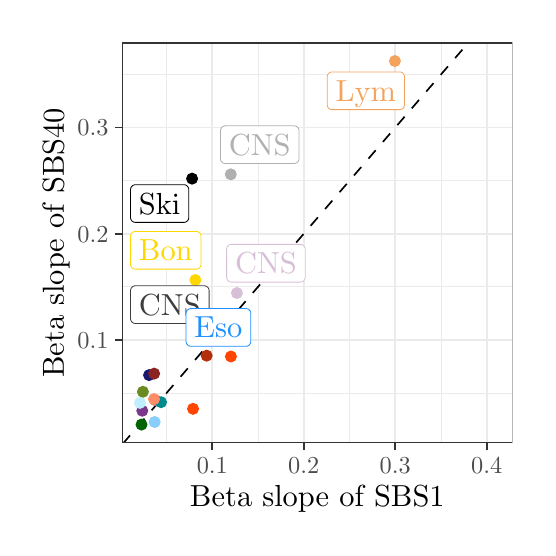
\begin{tikzpicture}[x=1pt,y=1pt]
\definecolor{fillColor}{RGB}{255,255,255}
\path[use as bounding box,fill=fillColor,fill opacity=0.00] (0,0) rectangle (180.67,180.67);
\begin{scope}
\path[clip] (  0.00,  0.00) rectangle (180.67,180.67);
\definecolor{drawColor}{RGB}{255,255,255}
\definecolor{fillColor}{RGB}{255,255,255}

\path[draw=drawColor,line width= 0.6pt,line join=round,line cap=round,fill=fillColor] (  0.00,  0.00) rectangle (180.68,180.68);
\end{scope}
\begin{scope}
\path[clip] ( 34.16, 30.69) rectangle (175.17,175.17);
\definecolor{fillColor}{RGB}{255,255,255}

\path[fill=fillColor] ( 34.16, 30.69) rectangle (175.17,175.17);
\definecolor{drawColor}{gray}{0.92}

\path[draw=drawColor,line width= 0.3pt,line join=round] ( 34.16, 48.66) --
	(175.17, 48.66);

\path[draw=drawColor,line width= 0.3pt,line join=round] ( 34.16, 87.04) --
	(175.17, 87.04);

\path[draw=drawColor,line width= 0.3pt,line join=round] ( 34.16,125.41) --
	(175.17,125.41);

\path[draw=drawColor,line width= 0.3pt,line join=round] ( 34.16,163.79) --
	(175.17,163.79);

\path[draw=drawColor,line width= 0.3pt,line join=round] ( 50.19, 30.69) --
	( 50.19,175.17);

\path[draw=drawColor,line width= 0.3pt,line join=round] ( 83.25, 30.69) --
	( 83.25,175.17);

\path[draw=drawColor,line width= 0.3pt,line join=round] (116.31, 30.69) --
	(116.31,175.17);

\path[draw=drawColor,line width= 0.3pt,line join=round] (149.37, 30.69) --
	(149.37,175.17);

\path[draw=drawColor,line width= 0.6pt,line join=round] ( 34.16, 67.85) --
	(175.17, 67.85);

\path[draw=drawColor,line width= 0.6pt,line join=round] ( 34.16,106.23) --
	(175.17,106.23);

\path[draw=drawColor,line width= 0.6pt,line join=round] ( 34.16,144.60) --
	(175.17,144.60);

\path[draw=drawColor,line width= 0.6pt,line join=round] ( 66.72, 30.69) --
	( 66.72,175.17);

\path[draw=drawColor,line width= 0.6pt,line join=round] ( 99.78, 30.69) --
	( 99.78,175.17);

\path[draw=drawColor,line width= 0.6pt,line join=round] (132.84, 30.69) --
	(132.84,175.17);

\path[draw=drawColor,line width= 0.6pt,line join=round] (165.90, 30.69) --
	(165.90,175.17);
\definecolor{drawColor}{RGB}{0,0,0}

\path[draw=drawColor,line width= 0.6pt,dash pattern=on 4pt off 4pt ,line join=round] (  8.26,  0.00) -- (163.92,180.67);
\definecolor{drawColor}{RGB}{255,215,0}
\definecolor{fillColor}{RGB}{255,215,0}

\path[draw=drawColor,line width= 0.4pt,line join=round,line cap=round,fill=fillColor] ( 60.59, 89.48) circle (  1.96);
\definecolor{drawColor}{RGB}{205,96,144}
\definecolor{fillColor}{RGB}{205,96,144}

\path[draw=drawColor,line width= 0.4pt,line join=round,line cap=round,fill=fillColor] ( 46.21, 46.02) circle (  1.96);
\definecolor{drawColor}{gray}{0.24}
\definecolor{fillColor}{gray}{0.24}

\path[draw=drawColor,line width= 0.4pt,line join=round,line cap=round,fill=fillColor] ( 61.35, 78.97) circle (  1.96);
\definecolor{drawColor}{RGB}{216,191,216}
\definecolor{fillColor}{RGB}{216,191,216}

\path[draw=drawColor,line width= 0.4pt,line join=round,line cap=round,fill=fillColor] ( 75.61, 84.79) circle (  1.96);
\definecolor{drawColor}{gray}{0.69}
\definecolor{fillColor}{gray}{0.69}

\path[draw=drawColor,line width= 0.4pt,line join=round,line cap=round,fill=fillColor] ( 73.40,127.67) circle (  1.96);
\definecolor{drawColor}{RGB}{25,25,112}
\definecolor{fillColor}{RGB}{25,25,112}

\path[draw=drawColor,line width= 0.4pt,line join=round,line cap=round,fill=fillColor] ( 43.85, 55.12) circle (  1.96);
\definecolor{drawColor}{RGB}{30,144,255}
\definecolor{fillColor}{RGB}{30,144,255}

\path[draw=drawColor,line width= 0.4pt,line join=round,line cap=round,fill=fillColor] ( 64.22, 77.20) circle (  1.96);
\definecolor{drawColor}{RGB}{139,35,35}
\definecolor{fillColor}{RGB}{139,35,35}

\path[draw=drawColor,line width= 0.4pt,line join=round,line cap=round,fill=fillColor] ( 45.70, 55.66) circle (  1.96);
\definecolor{drawColor}{RGB}{179,47,11}
\definecolor{fillColor}{RGB}{179,47,11}

\path[draw=drawColor,line width= 0.4pt,line join=round,line cap=round,fill=fillColor] ( 64.68, 62.15) circle (  1.96);
\definecolor{drawColor}{RGB}{255,69,0}
\definecolor{fillColor}{RGB}{255,69,0}

\path[draw=drawColor,line width= 0.4pt,line join=round,line cap=round,fill=fillColor] ( 73.44, 61.85) circle (  1.96);

\path[draw=drawColor,line width= 0.4pt,line join=round,line cap=round,fill=fillColor] ( 59.75, 42.94) circle (  1.96);
\definecolor{drawColor}{RGB}{0,100,0}
\definecolor{fillColor}{RGB}{0,100,0}

\path[draw=drawColor,line width= 0.4pt,line join=round,line cap=round,fill=fillColor] ( 41.14, 37.25) circle (  1.96);
\definecolor{drawColor}{RGB}{105,139,34}
\definecolor{fillColor}{RGB}{105,139,34}

\path[draw=drawColor,line width= 0.4pt,line join=round,line cap=round,fill=fillColor] ( 41.64, 49.10) circle (  1.96);
\definecolor{drawColor}{RGB}{244,163,93}
\definecolor{fillColor}{RGB}{244,163,93}

\path[draw=drawColor,line width= 0.4pt,line join=round,line cap=round,fill=fillColor] (132.69,168.61) circle (  1.96);
\definecolor{drawColor}{RGB}{0,139,139}
\definecolor{fillColor}{RGB}{0,139,139}

\path[draw=drawColor,line width= 0.4pt,line join=round,line cap=round,fill=fillColor] ( 48.19, 45.33) circle (  1.96);
\definecolor{drawColor}{RGB}{122,55,139}
\definecolor{fillColor}{RGB}{122,55,139}

\path[draw=drawColor,line width= 0.4pt,line join=round,line cap=round,fill=fillColor] ( 41.41, 42.24) circle (  1.96);
\definecolor{drawColor}{RGB}{135,206,250}
\definecolor{fillColor}{RGB}{135,206,250}

\path[draw=drawColor,line width= 0.4pt,line join=round,line cap=round,fill=fillColor] ( 45.89, 38.17) circle (  1.96);
\definecolor{drawColor}{RGB}{0,0,0}
\definecolor{fillColor}{RGB}{0,0,0}

\path[draw=drawColor,line width= 0.4pt,line join=round,line cap=round,fill=fillColor] ( 59.41,126.12) circle (  1.96);
\definecolor{drawColor}{RGB}{191,239,255}
\definecolor{fillColor}{RGB}{191,239,255}

\path[draw=drawColor,line width= 0.4pt,line join=round,line cap=round,fill=fillColor] ( 40.57, 45.08) circle (  1.96);
\definecolor{drawColor}{RGB}{147,112,219}
\definecolor{fillColor}{RGB}{147,112,219}

\path[draw=drawColor,line width= 0.4pt,line join=round,line cap=round,fill=fillColor] ( 72.64, 67.78) circle (  1.96);
\definecolor{drawColor}{RGB}{255,140,105}
\definecolor{fillColor}{RGB}{255,140,105}

\path[draw=drawColor,line width= 0.4pt,line join=round,line cap=round,fill=fillColor] ( 45.65, 46.46) circle (  1.96);
\end{scope}
\begin{scope}
\path[clip] ( 34.16, 30.69) rectangle (175.17,175.17);
\definecolor{drawColor}{RGB}{255,215,0}
\definecolor{fillColor}{RGB}{255,255,255}

\path[draw=drawColor,line width= 0.3pt,line join=round,line cap=round,fill=fillColor] ( 38.97, 93.42) --
	( 60.85, 93.42) --
	( 60.78, 93.42) --
	( 61.07, 93.43) --
	( 61.35, 93.49) --
	( 61.63, 93.59) --
	( 61.88, 93.74) --
	( 62.10, 93.92) --
	( 62.30, 94.14) --
	( 62.45, 94.39) --
	( 62.57, 94.65) --
	( 62.64, 94.94) --
	( 62.66, 95.22) --
	( 62.66, 95.22) --
	( 62.66,105.24) --
	( 62.66,105.24) --
	( 62.64,105.53) --
	( 62.57,105.81) --
	( 62.45,106.08) --
	( 62.30,106.32) --
	( 62.10,106.54) --
	( 61.88,106.72) --
	( 61.63,106.87) --
	( 61.35,106.97) --
	( 61.07,107.03) --
	( 60.85,107.04) --
	( 38.97,107.04) --
	( 39.19,107.03) --
	( 38.90,107.04) --
	( 38.61,107.01) --
	( 38.33,106.93) --
	( 38.07,106.80) --
	( 37.83,106.64) --
	( 37.62,106.44) --
	( 37.45,106.20) --
	( 37.31,105.95) --
	( 37.22,105.67) --
	( 37.17,105.38) --
	( 37.17,105.24) --
	( 37.17, 95.22) --
	( 37.17, 95.37) --
	( 37.17, 95.08) --
	( 37.22, 94.79) --
	( 37.31, 94.52) --
	( 37.45, 94.26) --
	( 37.62, 94.03) --
	( 37.83, 93.83) --
	( 38.07, 93.66) --
	( 38.33, 93.54) --
	( 38.61, 93.45) --
	( 38.90, 93.42) --
	cycle;
\end{scope}
\begin{scope}
\path[clip] ( 34.16, 30.69) rectangle (175.17,175.17);
\definecolor{drawColor}{RGB}{255,215,0}

\node[text=drawColor,anchor=base,inner sep=0pt, outer sep=0pt, scale=  1.10] at ( 49.91, 96.43) {Bon};
\definecolor{drawColor}{gray}{0.24}
\definecolor{fillColor}{RGB}{255,255,255}

\path[draw=drawColor,line width= 0.3pt,line join=round,line cap=round,fill=fillColor] ( 38.97, 73.77) --
	( 63.76, 73.77) --
	( 63.69, 73.77) --
	( 63.98, 73.78) --
	( 64.27, 73.84) --
	( 64.54, 73.94) --
	( 64.79, 74.09) --
	( 65.02, 74.27) --
	( 65.21, 74.49) --
	( 65.36, 74.74) --
	( 65.48, 75.00) --
	( 65.55, 75.29) --
	( 65.57, 75.58) --
	( 65.57, 75.58) --
	( 65.57, 85.59) --
	( 65.57, 85.59) --
	( 65.55, 85.88) --
	( 65.48, 86.16) --
	( 65.36, 86.43) --
	( 65.21, 86.67) --
	( 65.02, 86.89) --
	( 64.79, 87.07) --
	( 64.54, 87.22) --
	( 64.27, 87.32) --
	( 63.98, 87.38) --
	( 63.76, 87.39) --
	( 38.97, 87.39) --
	( 39.19, 87.38) --
	( 38.90, 87.39) --
	( 38.61, 87.36) --
	( 38.33, 87.28) --
	( 38.07, 87.15) --
	( 37.83, 86.99) --
	( 37.62, 86.79) --
	( 37.45, 86.55) --
	( 37.31, 86.30) --
	( 37.22, 86.02) --
	( 37.17, 85.73) --
	( 37.17, 85.59) --
	( 37.17, 75.58) --
	( 37.17, 75.72) --
	( 37.17, 75.43) --
	( 37.22, 75.14) --
	( 37.31, 74.87) --
	( 37.45, 74.61) --
	( 37.62, 74.38) --
	( 37.83, 74.18) --
	( 38.07, 74.01) --
	( 38.33, 73.89) --
	( 38.61, 73.81) --
	( 38.90, 73.77) --
	cycle;
\end{scope}
\begin{scope}
\path[clip] ( 34.16, 30.69) rectangle (175.17,175.17);
\definecolor{drawColor}{gray}{0.24}

\node[text=drawColor,anchor=base,inner sep=0pt, outer sep=0pt, scale=  1.10] at ( 51.37, 76.78) {CNS};
\definecolor{drawColor}{RGB}{216,191,216}
\definecolor{fillColor}{RGB}{255,255,255}

\path[draw=drawColor,line width= 0.3pt,line join=round,line cap=round,fill=fillColor] ( 73.70, 88.72) --
	( 98.49, 88.72) --
	( 98.41, 88.72) --
	( 98.70, 88.74) --
	( 98.99, 88.79) --
	( 99.26, 88.90) --
	( 99.51, 89.04) --
	( 99.74, 89.23) --
	( 99.93, 89.44) --
	(100.09, 89.69) --
	(100.20, 89.96) --
	(100.27, 90.24) --
	(100.29, 90.53) --
	(100.29, 90.53) --
	(100.29,100.54) --
	(100.29,100.54) --
	(100.27,100.83) --
	(100.20,101.11) --
	(100.09,101.38) --
	( 99.93,101.63) --
	( 99.74,101.84) --
	( 99.51,102.03) --
	( 99.26,102.17) --
	( 98.99,102.28) --
	( 98.70,102.34) --
	( 98.49,102.35) --
	( 73.70,102.35) --
	( 73.91,102.34) --
	( 73.62,102.35) --
	( 73.33,102.31) --
	( 73.06,102.23) --
	( 72.79,102.11) --
	( 72.55,101.94) --
	( 72.34,101.74) --
	( 72.17,101.51) --
	( 72.03,101.25) --
	( 71.94,100.97) --
	( 71.89,100.69) --
	( 71.89,100.54) --
	( 71.89, 90.53) --
	( 71.89, 90.67) --
	( 71.89, 90.38) --
	( 71.94, 90.10) --
	( 72.03, 89.82) --
	( 72.17, 89.56) --
	( 72.34, 89.33) --
	( 72.55, 89.13) --
	( 72.79, 88.96) --
	( 73.06, 88.84) --
	( 73.33, 88.76) --
	( 73.62, 88.72) --
	cycle;
\end{scope}
\begin{scope}
\path[clip] ( 34.16, 30.69) rectangle (175.17,175.17);
\definecolor{drawColor}{RGB}{216,191,216}

\node[text=drawColor,anchor=base,inner sep=0pt, outer sep=0pt, scale=  1.10] at ( 86.09, 91.73) {CNS};
\definecolor{drawColor}{gray}{0.69}
\definecolor{fillColor}{RGB}{255,255,255}

\path[draw=drawColor,line width= 0.3pt,line join=round,line cap=round,fill=fillColor] ( 71.47,131.58) --
	( 96.26,131.58) --
	( 96.18,131.58) --
	( 96.47,131.59) --
	( 96.76,131.65) --
	( 97.03,131.75) --
	( 97.28,131.90) --
	( 97.51,132.08) --
	( 97.70,132.30) --
	( 97.86,132.55) --
	( 97.97,132.81) --
	( 98.04,133.10) --
	( 98.06,133.38) --
	( 98.06,133.38) --
	( 98.06,143.40) --
	( 98.06,143.40) --
	( 98.04,143.69) --
	( 97.97,143.97) --
	( 97.86,144.24) --
	( 97.70,144.48) --
	( 97.51,144.70) --
	( 97.28,144.88) --
	( 97.03,145.03) --
	( 96.76,145.13) --
	( 96.47,145.19) --
	( 96.26,145.20) --
	( 71.47,145.20) --
	( 71.68,145.19) --
	( 71.39,145.20) --
	( 71.11,145.17) --
	( 70.83,145.09) --
	( 70.56,144.96) --
	( 70.32,144.80) --
	( 70.11,144.60) --
	( 69.94,144.36) --
	( 69.80,144.11) --
	( 69.71,143.83) --
	( 69.67,143.54) --
	( 69.66,143.40) --
	( 69.66,133.38) --
	( 69.67,133.53) --
	( 69.67,133.24) --
	( 69.71,132.95) --
	( 69.80,132.68) --
	( 69.94,132.42) --
	( 70.11,132.19) --
	( 70.32,131.99) --
	( 70.56,131.82) --
	( 70.83,131.70) --
	( 71.11,131.61) --
	( 71.39,131.58) --
	cycle;
\end{scope}
\begin{scope}
\path[clip] ( 34.16, 30.69) rectangle (175.17,175.17);
\definecolor{drawColor}{gray}{0.69}

\node[text=drawColor,anchor=base,inner sep=0pt, outer sep=0pt, scale=  1.10] at ( 83.86,134.59) {CNS};
\definecolor{drawColor}{RGB}{30,144,255}
\definecolor{fillColor}{RGB}{255,255,255}

\path[draw=drawColor,line width= 0.3pt,line join=round,line cap=round,fill=fillColor] ( 59.03, 65.54) --
	( 78.83, 65.54) --
	( 78.75, 65.54) --
	( 79.05, 65.55) --
	( 79.33, 65.61) --
	( 79.60, 65.71) --
	( 79.85, 65.86) --
	( 80.08, 66.04) --
	( 80.27, 66.26) --
	( 80.43, 66.51) --
	( 80.54, 66.77) --
	( 80.61, 67.06) --
	( 80.63, 67.35) --
	( 80.63, 67.35) --
	( 80.63, 77.36) --
	( 80.63, 77.36) --
	( 80.61, 77.65) --
	( 80.54, 77.93) --
	( 80.43, 78.20) --
	( 80.27, 78.44) --
	( 80.08, 78.66) --
	( 79.85, 78.85) --
	( 79.60, 78.99) --
	( 79.33, 79.09) --
	( 79.05, 79.15) --
	( 78.83, 79.17) --
	( 59.03, 79.17) --
	( 59.25, 79.15) --
	( 58.96, 79.16) --
	( 58.67, 79.13) --
	( 58.39, 79.05) --
	( 58.13, 78.92) --
	( 57.89, 78.76) --
	( 57.68, 78.56) --
	( 57.51, 78.32) --
	( 57.37, 78.07) --
	( 57.28, 77.79) --
	( 57.23, 77.50) --
	( 57.23, 77.36) --
	( 57.23, 67.35) --
	( 57.23, 67.49) --
	( 57.23, 67.20) --
	( 57.28, 66.91) --
	( 57.37, 66.64) --
	( 57.51, 66.38) --
	( 57.68, 66.15) --
	( 57.89, 65.95) --
	( 58.13, 65.78) --
	( 58.39, 65.66) --
	( 58.67, 65.58) --
	( 58.96, 65.54) --
	cycle;
\end{scope}
\begin{scope}
\path[clip] ( 34.16, 30.69) rectangle (175.17,175.17);
\definecolor{drawColor}{RGB}{30,144,255}

\node[text=drawColor,anchor=base,inner sep=0pt, outer sep=0pt, scale=  1.10] at ( 68.93, 68.55) {Eso};
\definecolor{drawColor}{RGB}{244,163,93}
\definecolor{fillColor}{RGB}{255,255,255}

\path[draw=drawColor,line width= 0.3pt,line join=round,line cap=round,fill=fillColor] (110.04,151.06) --
	(134.37,151.06) --
	(134.30,151.06) --
	(134.59,151.07) --
	(134.87,151.13) --
	(135.15,151.23) --
	(135.40,151.38) --
	(135.62,151.56) --
	(135.82,151.78) --
	(135.97,152.02) --
	(136.08,152.29) --
	(136.15,152.57) --
	(136.18,152.86) --
	(136.18,152.86) --
	(136.18,162.88) --
	(136.18,162.88) --
	(136.15,163.16) --
	(136.08,163.45) --
	(135.97,163.71) --
	(135.82,163.96) --
	(135.62,164.18) --
	(135.40,164.36) --
	(135.15,164.51) --
	(134.87,164.61) --
	(134.59,164.67) --
	(134.37,164.68) --
	(110.04,164.68) --
	(110.26,164.67) --
	(109.97,164.68) --
	(109.68,164.65) --
	(109.40,164.56) --
	(109.14,164.44) --
	(108.90,164.27) --
	(108.69,164.07) --
	(108.51,163.84) --
	(108.38,163.58) --
	(108.29,163.31) --
	(108.24,163.02) --
	(108.23,162.88) --
	(108.23,152.86) --
	(108.24,153.01) --
	(108.24,152.72) --
	(108.29,152.43) --
	(108.38,152.15) --
	(108.51,151.90) --
	(108.69,151.66) --
	(108.90,151.46) --
	(109.14,151.30) --
	(109.40,151.17) --
	(109.68,151.09) --
	(109.97,151.06) --
	cycle;
\end{scope}
\begin{scope}
\path[clip] ( 34.16, 30.69) rectangle (175.17,175.17);
\definecolor{drawColor}{RGB}{244,163,93}

\node[text=drawColor,anchor=base,inner sep=0pt, outer sep=0pt, scale=  1.10] at (122.21,154.07) {Lym};
\definecolor{drawColor}{RGB}{0,0,0}
\definecolor{fillColor}{RGB}{255,255,255}

\path[draw=drawColor,line width= 0.3pt,line join=round,line cap=round,fill=fillColor] ( 38.97,110.31) --
	( 56.41,110.31) --
	( 56.33,110.31) --
	( 56.62,110.32) --
	( 56.91,110.38) --
	( 57.18,110.48) --
	( 57.43,110.63) --
	( 57.66,110.81) --
	( 57.85,111.03) --
	( 58.01,111.27) --
	( 58.12,111.54) --
	( 58.19,111.82) --
	( 58.21,112.11) --
	( 58.21,112.11) --
	( 58.21,122.13) --
	( 58.21,122.13) --
	( 58.19,122.42) --
	( 58.12,122.70) --
	( 58.01,122.97) --
	( 57.85,123.21) --
	( 57.66,123.43) --
	( 57.43,123.61) --
	( 57.18,123.76) --
	( 56.91,123.86) --
	( 56.62,123.92) --
	( 56.41,123.93) --
	( 38.97,123.93) --
	( 39.19,123.92) --
	( 38.90,123.93) --
	( 38.61,123.90) --
	( 38.33,123.81) --
	( 38.07,123.69) --
	( 37.83,123.53) --
	( 37.62,123.32) --
	( 37.45,123.09) --
	( 37.31,122.83) --
	( 37.22,122.56) --
	( 37.17,122.27) --
	( 37.17,122.13) --
	( 37.17,112.11) --
	( 37.17,112.26) --
	( 37.17,111.97) --
	( 37.22,111.68) --
	( 37.31,111.40) --
	( 37.45,111.15) --
	( 37.62,110.91) --
	( 37.83,110.71) --
	( 38.07,110.55) --
	( 38.33,110.42) --
	( 38.61,110.34) --
	( 38.90,110.31) --
	cycle;
\end{scope}
\begin{scope}
\path[clip] ( 34.16, 30.69) rectangle (175.17,175.17);
\definecolor{drawColor}{RGB}{0,0,0}

\node[text=drawColor,anchor=base,inner sep=0pt, outer sep=0pt, scale=  1.10] at ( 47.69,113.32) {Ski};
\definecolor{drawColor}{gray}{0.20}

\path[draw=drawColor,line width= 0.6pt,line join=round,line cap=round] ( 34.16, 30.69) rectangle (175.17,175.17);
\end{scope}
\begin{scope}
\path[clip] (  0.00,  0.00) rectangle (180.67,180.67);
\definecolor{drawColor}{gray}{0.30}

\node[text=drawColor,anchor=base east,inner sep=0pt, outer sep=0pt, scale=  0.88] at ( 29.21, 64.82) {0.1};

\node[text=drawColor,anchor=base east,inner sep=0pt, outer sep=0pt, scale=  0.88] at ( 29.21,103.20) {0.2};

\node[text=drawColor,anchor=base east,inner sep=0pt, outer sep=0pt, scale=  0.88] at ( 29.21,141.57) {0.3};
\end{scope}
\begin{scope}
\path[clip] (  0.00,  0.00) rectangle (180.67,180.67);
\definecolor{drawColor}{gray}{0.20}

\path[draw=drawColor,line width= 0.6pt,line join=round] ( 31.41, 67.85) --
	( 34.16, 67.85);

\path[draw=drawColor,line width= 0.6pt,line join=round] ( 31.41,106.23) --
	( 34.16,106.23);

\path[draw=drawColor,line width= 0.6pt,line join=round] ( 31.41,144.60) --
	( 34.16,144.60);
\end{scope}
\begin{scope}
\path[clip] (  0.00,  0.00) rectangle (180.67,180.67);
\definecolor{drawColor}{gray}{0.20}

\path[draw=drawColor,line width= 0.6pt,line join=round] ( 66.72, 27.94) --
	( 66.72, 30.69);

\path[draw=drawColor,line width= 0.6pt,line join=round] ( 99.78, 27.94) --
	( 99.78, 30.69);

\path[draw=drawColor,line width= 0.6pt,line join=round] (132.84, 27.94) --
	(132.84, 30.69);

\path[draw=drawColor,line width= 0.6pt,line join=round] (165.90, 27.94) --
	(165.90, 30.69);
\end{scope}
\begin{scope}
\path[clip] (  0.00,  0.00) rectangle (180.67,180.67);
\definecolor{drawColor}{gray}{0.30}

\node[text=drawColor,anchor=base,inner sep=0pt, outer sep=0pt, scale=  0.88] at ( 66.72, 19.68) {0.1};

\node[text=drawColor,anchor=base,inner sep=0pt, outer sep=0pt, scale=  0.88] at ( 99.78, 19.68) {0.2};

\node[text=drawColor,anchor=base,inner sep=0pt, outer sep=0pt, scale=  0.88] at (132.84, 19.68) {0.3};

\node[text=drawColor,anchor=base,inner sep=0pt, outer sep=0pt, scale=  0.88] at (165.90, 19.68) {0.4};
\end{scope}
\begin{scope}
\path[clip] (  0.00,  0.00) rectangle (180.67,180.67);
\definecolor{drawColor}{RGB}{0,0,0}

\node[text=drawColor,anchor=base,inner sep=0pt, outer sep=0pt, scale=  1.10] at (104.67,  7.64) {Beta slope of SBS1};
\end{scope}
\begin{scope}
\path[clip] (  0.00,  0.00) rectangle (180.67,180.67);
\definecolor{drawColor}{RGB}{0,0,0}

\node[text=drawColor,rotate= 90.00,anchor=base,inner sep=0pt, outer sep=0pt, scale=  1.10] at ( 13.08,102.93) {Beta slope of SBS40};
\end{scope}
\end{tikzpicture}
